\documentclass[]{article}
\usepackage{lmodern}
\usepackage{amssymb,amsmath}
\usepackage{ifxetex,ifluatex}
\usepackage{fixltx2e} % provides \textsubscript
\ifnum 0\ifxetex 1\fi\ifluatex 1\fi=0 % if pdftex
  \usepackage[T1]{fontenc}
  \usepackage[utf8]{inputenc}
\else % if luatex or xelatex
  \ifxetex
    \usepackage{mathspec}
  \else
    \usepackage{fontspec}
  \fi
  \defaultfontfeatures{Ligatures=TeX,Scale=MatchLowercase}
\fi
% use upquote if available, for straight quotes in verbatim environments
\IfFileExists{upquote.sty}{\usepackage{upquote}}{}
% use microtype if available
\IfFileExists{microtype.sty}{%
\usepackage{microtype}
\UseMicrotypeSet[protrusion]{basicmath} % disable protrusion for tt fonts
}{}
\usepackage[margin=1in]{geometry}
\usepackage{hyperref}
\hypersetup{unicode=true,
            pdftitle={Extra Figures},
            pdfborder={0 0 0},
            breaklinks=true}
\urlstyle{same}  % don't use monospace font for urls
\usepackage{color}
\usepackage{fancyvrb}
\newcommand{\VerbBar}{|}
\newcommand{\VERB}{\Verb[commandchars=\\\{\}]}
\DefineVerbatimEnvironment{Highlighting}{Verbatim}{commandchars=\\\{\}}
% Add ',fontsize=\small' for more characters per line
\usepackage{framed}
\definecolor{shadecolor}{RGB}{248,248,248}
\newenvironment{Shaded}{\begin{snugshade}}{\end{snugshade}}
\newcommand{\KeywordTok}[1]{\textcolor[rgb]{0.13,0.29,0.53}{\textbf{{#1}}}}
\newcommand{\DataTypeTok}[1]{\textcolor[rgb]{0.13,0.29,0.53}{{#1}}}
\newcommand{\DecValTok}[1]{\textcolor[rgb]{0.00,0.00,0.81}{{#1}}}
\newcommand{\BaseNTok}[1]{\textcolor[rgb]{0.00,0.00,0.81}{{#1}}}
\newcommand{\FloatTok}[1]{\textcolor[rgb]{0.00,0.00,0.81}{{#1}}}
\newcommand{\ConstantTok}[1]{\textcolor[rgb]{0.00,0.00,0.00}{{#1}}}
\newcommand{\CharTok}[1]{\textcolor[rgb]{0.31,0.60,0.02}{{#1}}}
\newcommand{\SpecialCharTok}[1]{\textcolor[rgb]{0.00,0.00,0.00}{{#1}}}
\newcommand{\StringTok}[1]{\textcolor[rgb]{0.31,0.60,0.02}{{#1}}}
\newcommand{\VerbatimStringTok}[1]{\textcolor[rgb]{0.31,0.60,0.02}{{#1}}}
\newcommand{\SpecialStringTok}[1]{\textcolor[rgb]{0.31,0.60,0.02}{{#1}}}
\newcommand{\ImportTok}[1]{{#1}}
\newcommand{\CommentTok}[1]{\textcolor[rgb]{0.56,0.35,0.01}{\textit{{#1}}}}
\newcommand{\DocumentationTok}[1]{\textcolor[rgb]{0.56,0.35,0.01}{\textbf{\textit{{#1}}}}}
\newcommand{\AnnotationTok}[1]{\textcolor[rgb]{0.56,0.35,0.01}{\textbf{\textit{{#1}}}}}
\newcommand{\CommentVarTok}[1]{\textcolor[rgb]{0.56,0.35,0.01}{\textbf{\textit{{#1}}}}}
\newcommand{\OtherTok}[1]{\textcolor[rgb]{0.56,0.35,0.01}{{#1}}}
\newcommand{\FunctionTok}[1]{\textcolor[rgb]{0.00,0.00,0.00}{{#1}}}
\newcommand{\VariableTok}[1]{\textcolor[rgb]{0.00,0.00,0.00}{{#1}}}
\newcommand{\ControlFlowTok}[1]{\textcolor[rgb]{0.13,0.29,0.53}{\textbf{{#1}}}}
\newcommand{\OperatorTok}[1]{\textcolor[rgb]{0.81,0.36,0.00}{\textbf{{#1}}}}
\newcommand{\BuiltInTok}[1]{{#1}}
\newcommand{\ExtensionTok}[1]{{#1}}
\newcommand{\PreprocessorTok}[1]{\textcolor[rgb]{0.56,0.35,0.01}{\textit{{#1}}}}
\newcommand{\AttributeTok}[1]{\textcolor[rgb]{0.77,0.63,0.00}{{#1}}}
\newcommand{\RegionMarkerTok}[1]{{#1}}
\newcommand{\InformationTok}[1]{\textcolor[rgb]{0.56,0.35,0.01}{\textbf{\textit{{#1}}}}}
\newcommand{\WarningTok}[1]{\textcolor[rgb]{0.56,0.35,0.01}{\textbf{\textit{{#1}}}}}
\newcommand{\AlertTok}[1]{\textcolor[rgb]{0.94,0.16,0.16}{{#1}}}
\newcommand{\ErrorTok}[1]{\textcolor[rgb]{0.64,0.00,0.00}{\textbf{{#1}}}}
\newcommand{\NormalTok}[1]{{#1}}
\usepackage{graphicx,grffile}
\makeatletter
\def\maxwidth{\ifdim\Gin@nat@width>\linewidth\linewidth\else\Gin@nat@width\fi}
\def\maxheight{\ifdim\Gin@nat@height>\textheight\textheight\else\Gin@nat@height\fi}
\makeatother
% Scale images if necessary, so that they will not overflow the page
% margins by default, and it is still possible to overwrite the defaults
% using explicit options in \includegraphics[width, height, ...]{}
\setkeys{Gin}{width=\maxwidth,height=\maxheight,keepaspectratio}
\IfFileExists{parskip.sty}{%
\usepackage{parskip}
}{% else
\setlength{\parindent}{0pt}
\setlength{\parskip}{6pt plus 2pt minus 1pt}
}
\setlength{\emergencystretch}{3em}  % prevent overfull lines
\providecommand{\tightlist}{%
  \setlength{\itemsep}{0pt}\setlength{\parskip}{0pt}}
\setcounter{secnumdepth}{0}
% Redefines (sub)paragraphs to behave more like sections
\ifx\paragraph\undefined\else
\let\oldparagraph\paragraph
\renewcommand{\paragraph}[1]{\oldparagraph{#1}\mbox{}}
\fi
\ifx\subparagraph\undefined\else
\let\oldsubparagraph\subparagraph
\renewcommand{\subparagraph}[1]{\oldsubparagraph{#1}\mbox{}}
\fi

%%% Use protect on footnotes to avoid problems with footnotes in titles
\let\rmarkdownfootnote\footnote%
\def\footnote{\protect\rmarkdownfootnote}

%%% Change title format to be more compact
\usepackage{titling}

% Create subtitle command for use in maketitle
\newcommand{\subtitle}[1]{
  \posttitle{
    \begin{center}\large#1\end{center}
    }
}

\setlength{\droptitle}{-2em}
  \title{Extra Figures}
  \pretitle{\vspace{\droptitle}\centering\huge}
  \posttitle{\par}
  \author{}
  \preauthor{}\postauthor{}
  \date{}
  \predate{}\postdate{}


\begin{document}
\maketitle

\begin{Shaded}
\begin{Highlighting}[]
\KeywordTok{library}\NormalTok{(raster)}
\end{Highlighting}
\end{Shaded}

\begin{verbatim}
## Loading required package: sp
\end{verbatim}

\begin{Shaded}
\begin{Highlighting}[]
\KeywordTok{library}\NormalTok{(rasterVis)}
\end{Highlighting}
\end{Shaded}

\begin{verbatim}
## Loading required package: lattice
\end{verbatim}

\begin{verbatim}
## Loading required package: latticeExtra
\end{verbatim}

\begin{verbatim}
## Loading required package: RColorBrewer
\end{verbatim}

\begin{Shaded}
\begin{Highlighting}[]
\KeywordTok{library}\NormalTok{(magrittr)}
\end{Highlighting}
\end{Shaded}

\begin{verbatim}
## 
## Attaching package: 'magrittr'
\end{verbatim}

\begin{verbatim}
## The following object is masked from 'package:raster':
## 
##     extract
\end{verbatim}

\begin{Shaded}
\begin{Highlighting}[]
\KeywordTok{brick}\NormalTok{(}\StringTok{'Data/b40.lm850-1850.1deg.001.cam2.h0.PRECT.085001-185012.nc'}\NormalTok{) %>%}\StringTok{ }
\StringTok{  }\KeywordTok{extract2}\NormalTok{(}\DecValTok{1}\NormalTok{) %>%}\StringTok{ }
\StringTok{  }\NormalTok{rotate %>%}
\StringTok{  }\KeywordTok{multiply_by}\NormalTok{(}\FloatTok{2.628e+9}\NormalTok{) %>%}
\StringTok{  }\KeywordTok{levelplot}\NormalTok{(}\DataTypeTok{margin =} \NormalTok{F, }\DataTypeTok{par.settings =} \KeywordTok{BTCTheme}\NormalTok{(), }\DataTypeTok{colorkey =} \NormalTok{F, }\DataTypeTok{xlab=}\OtherTok{NULL}\NormalTok{, }\DataTypeTok{ylab=}\OtherTok{NULL}\NormalTok{, }\DataTypeTok{scales=}\KeywordTok{list}\NormalTok{(}\DataTypeTok{draw=}\OtherTok{FALSE}\NormalTok{))}
\end{Highlighting}
\end{Shaded}

\begin{verbatim}
## Loading required namespace: ncdf4
\end{verbatim}

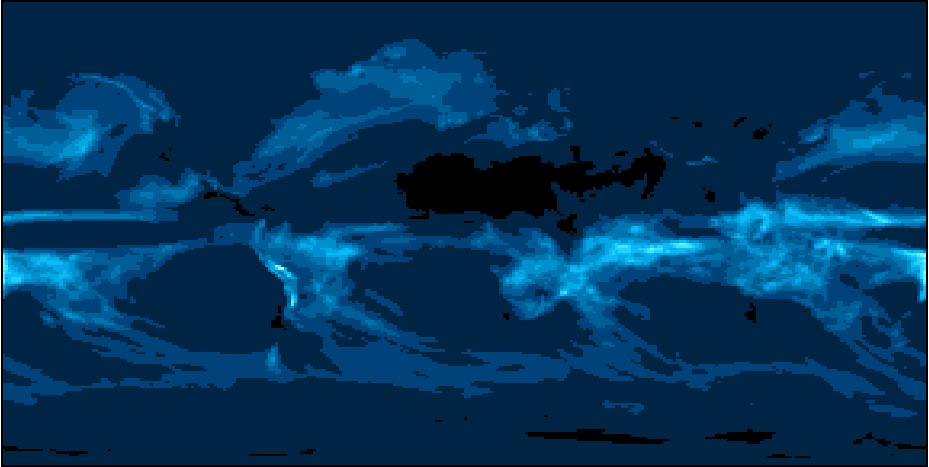
\includegraphics{extra-figures_files/figure-latex/unnamed-chunk-2-1.pdf}

\begin{Shaded}
\begin{Highlighting}[]
\KeywordTok{mean}\NormalTok{((}\KeywordTok{brick}\NormalTok{(}\StringTok{'Data/b40.lm850-1850.1deg.001.cam2.h0.TREFMNAV.085001-185012.nc'}\NormalTok{) %>%}
\StringTok{  }\KeywordTok{extract2}\NormalTok{(}\DecValTok{1}\NormalTok{) %>%}
\StringTok{  }\NormalTok{rotate %>%}
\StringTok{  }\KeywordTok{subtract}\NormalTok{(}\FloatTok{273.15}\NormalTok{)),}
\NormalTok{(}\KeywordTok{brick}\NormalTok{(}\StringTok{'Data/b40.lm850-1850.1deg.001.cam2.h0.TREFMXAV.085001-185012.nc'}\NormalTok{) %>%}
\StringTok{  }\KeywordTok{extract2}\NormalTok{(}\DecValTok{1}\NormalTok{) %>%}
\StringTok{  }\NormalTok{rotate %>%}
\StringTok{  }\KeywordTok{subtract}\NormalTok{(}\FloatTok{273.15}\NormalTok{))) %>%}
\StringTok{  }\KeywordTok{levelplot}\NormalTok{(}\DataTypeTok{margin =} \NormalTok{F, }\DataTypeTok{par.settings =} \KeywordTok{BuRdTheme}\NormalTok{(), }\DataTypeTok{colorkey =} \NormalTok{F,}\DataTypeTok{xlab=}\OtherTok{NULL}\NormalTok{, }\DataTypeTok{ylab=}\OtherTok{NULL}\NormalTok{, }\DataTypeTok{scales=}\KeywordTok{list}\NormalTok{(}\DataTypeTok{draw=}\OtherTok{FALSE}\NormalTok{))}
\end{Highlighting}
\end{Shaded}

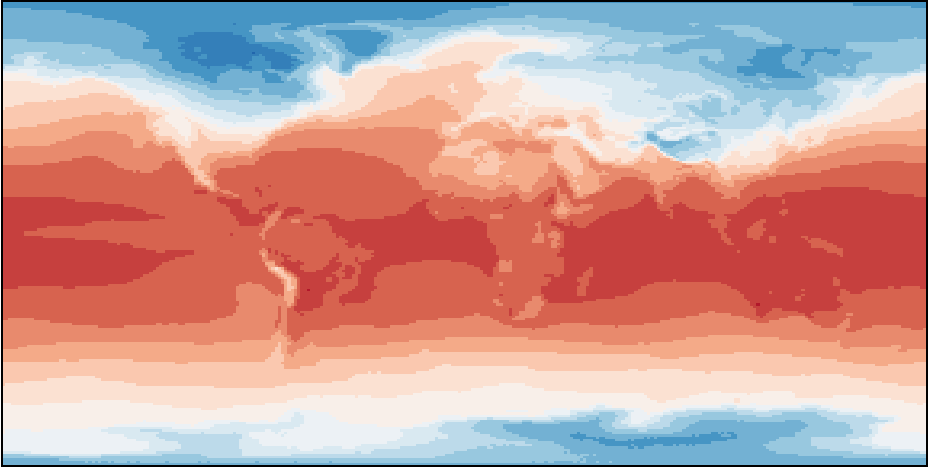
\includegraphics{extra-figures_files/figure-latex/unnamed-chunk-2-2.pdf}

\begin{Shaded}
\begin{Highlighting}[]
\KeywordTok{library}\NormalTok{(maps)}
\KeywordTok{library}\NormalTok{(maptools)}
\end{Highlighting}
\end{Shaded}

\begin{verbatim}
## Checking rgeos availability: TRUE
\end{verbatim}

\begin{Shaded}
\begin{Highlighting}[]
\NormalTok{states.ply <-}\StringTok{ }\NormalTok{maps::}\KeywordTok{map}\NormalTok{(}\StringTok{'state'}\NormalTok{, }\DataTypeTok{region =} \KeywordTok{c}\NormalTok{(}\StringTok{'arizona'}\NormalTok{, }\StringTok{'new mexico'}\NormalTok{), }\DataTypeTok{fill =} \NormalTok{T, }\DataTypeTok{plot =} \NormalTok{F)}
\NormalTok{IDs <-}\StringTok{ }\KeywordTok{sapply}\NormalTok{(}\KeywordTok{strsplit}\NormalTok{(states.ply$names, }\StringTok{":"}\NormalTok{), function(x) x[}\DecValTok{1}\NormalTok{])}
\NormalTok{states.ply <-}\StringTok{ }\KeywordTok{map2SpatialPolygons}\NormalTok{(states.ply, }\DataTypeTok{IDs=}\NormalTok{IDs)}
\CommentTok{#assumes you have water stress map from sw_variability scitp}
\NormalTok{ws.map <-}\StringTok{ }\KeywordTok{brick}\NormalTok{(}\StringTok{'Data/water_stress.nc'}\NormalTok{)}
\NormalTok{ws.map.plot <-}\StringTok{ }\KeywordTok{disaggregate}\NormalTok{(ws.map[[}\DecValTok{1}\NormalTok{:}\DecValTok{12}\NormalTok{]],}\DataTypeTok{fac =} \DecValTok{5}\NormalTok{, }\DataTypeTok{method =} \StringTok{'bilinear'}\NormalTok{) %>%}\StringTok{ }\KeywordTok{mask}\NormalTok{(states.ply)}
\KeywordTok{levelplot}\NormalTok{(ws.map.plot, }\DataTypeTok{names.attr =} \NormalTok{month.name, }\DataTypeTok{at =} \KeywordTok{seq}\NormalTok{(-}\DecValTok{250}\NormalTok{,}\DecValTok{250}\NormalTok{, }\DecValTok{15}\NormalTok{), }\DataTypeTok{xlab=}\OtherTok{NULL}\NormalTok{, }\DataTypeTok{ylab=}\OtherTok{NULL}\NormalTok{, }\DataTypeTok{scales=}\KeywordTok{list}\NormalTok{(}\DataTypeTok{draw=}\OtherTok{FALSE}\NormalTok{), }\DataTypeTok{par.settings =} \KeywordTok{PuOrTheme}\NormalTok{(}\DataTypeTok{axis.line =} \KeywordTok{list}\NormalTok{(}\DataTypeTok{col =} \StringTok{"transparent"}\NormalTok{)), }\DataTypeTok{layout =} \KeywordTok{c}\NormalTok{(}\DecValTok{4}\NormalTok{,}\DecValTok{3}\NormalTok{)) +}
\StringTok{  }\KeywordTok{layer}\NormalTok{(}\KeywordTok{sp.polygons}\NormalTok{(states.ply))}
\end{Highlighting}
\end{Shaded}

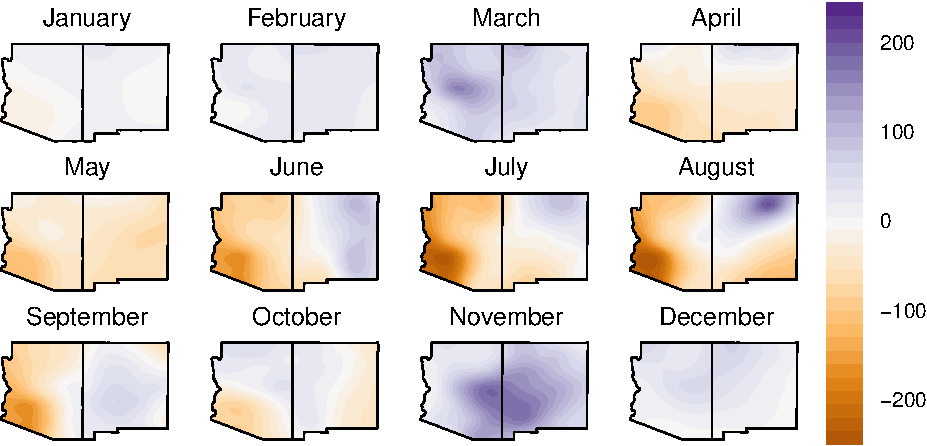
\includegraphics{extra-figures_files/figure-latex/water_stress-1.pdf}

\begin{Shaded}
\begin{Highlighting}[]
\KeywordTok{levelplot}\NormalTok{(ws.map.plot, }\DataTypeTok{names.attr =} \NormalTok{month.name, }\DataTypeTok{at =} \KeywordTok{seq}\NormalTok{(-}\DecValTok{250}\NormalTok{,}\DecValTok{250}\NormalTok{, }\DecValTok{25}\NormalTok{), }\DataTypeTok{xlab=}\OtherTok{NULL}\NormalTok{, }\DataTypeTok{ylab=}\OtherTok{NULL}\NormalTok{, }\DataTypeTok{scales=}\KeywordTok{list}\NormalTok{(}\DataTypeTok{draw=}\OtherTok{FALSE}\NormalTok{), }\DataTypeTok{par.settings =} \KeywordTok{PuOrTheme}\NormalTok{(}\DataTypeTok{axis.line =} \KeywordTok{list}\NormalTok{(}\DataTypeTok{col =} \StringTok{"transparent"}\NormalTok{))) +}
\StringTok{  }\KeywordTok{layer}\NormalTok{(}\KeywordTok{sp.polygons}\NormalTok{(states.ply))}
\end{Highlighting}
\end{Shaded}

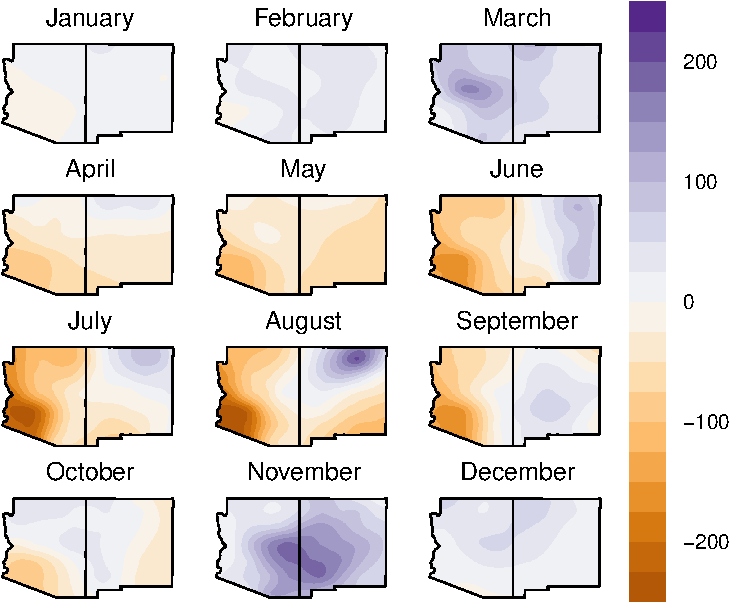
\includegraphics{extra-figures_files/figure-latex/water_stress-2.pdf}

\begin{Shaded}
\begin{Highlighting}[]
\NormalTok{eof.all <-}\StringTok{ }\KeywordTok{brick}\NormalTok{(}\StringTok{'Data/eof_all.nc'}\NormalTok{)[[}\DecValTok{1}\NormalTok{:}\DecValTok{6}\NormalTok{]] %>%}\StringTok{ }\KeywordTok{mask}\NormalTok{(states.ply) %>%}\StringTok{ }\KeywordTok{disaggregate}\NormalTok{(}\DataTypeTok{fac=}\DecValTok{10}\NormalTok{, }\DataTypeTok{method =} \StringTok{'bilinear'}\NormalTok{)}
\KeywordTok{names}\NormalTok{(eof.all) <-}\StringTok{ }\KeywordTok{c}\NormalTok{(}\StringTok{'EOF1'}\NormalTok{, }\StringTok{'EOF2'}\NormalTok{, }\StringTok{'EOF3'}\NormalTok{, }\StringTok{'EOF4'}\NormalTok{, }\StringTok{'EOF5'}\NormalTok{, }\StringTok{'EOF6'}\NormalTok{)}
\KeywordTok{levelplot}\NormalTok{(eof.all, }\DataTypeTok{par.settings =} \KeywordTok{RdBuTheme}\NormalTok{(}\DataTypeTok{axis.line =} \KeywordTok{list}\NormalTok{(}\DataTypeTok{col =} \StringTok{"transparent"}\NormalTok{)), }\DataTypeTok{xlab=}\OtherTok{NULL}\NormalTok{, }\DataTypeTok{ylab=}\OtherTok{NULL}\NormalTok{, }\DataTypeTok{scales=}\KeywordTok{list}\NormalTok{(}\DataTypeTok{draw=}\OtherTok{FALSE}\NormalTok{), }\DataTypeTok{at =} \KeywordTok{seq}\NormalTok{(-.}\DecValTok{029}\NormalTok{,.}\DecValTok{029}\NormalTok{,.}\DecValTok{0029}\NormalTok{), }\DataTypeTok{layout =} \KeywordTok{c}\NormalTok{(}\DecValTok{3}\NormalTok{,}\DecValTok{2}\NormalTok{)) +}
\StringTok{  }\KeywordTok{layer}\NormalTok{(}\KeywordTok{sp.polygons}\NormalTok{(states.ply))}
\end{Highlighting}
\end{Shaded}

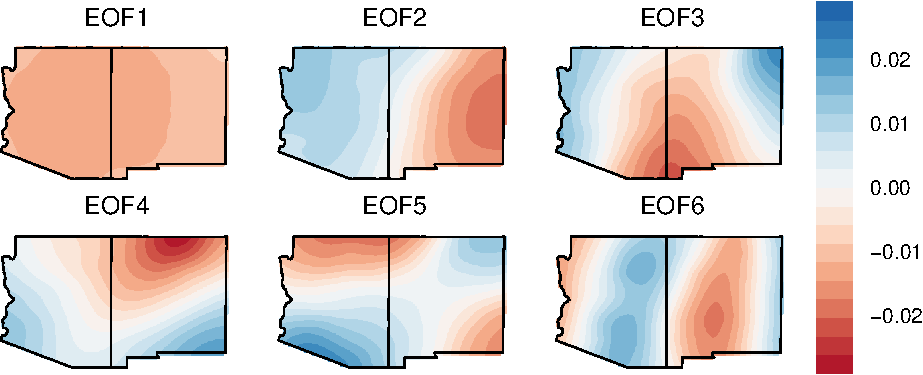
\includegraphics{extra-figures_files/figure-latex/eofs-1.pdf}


\end{document}
